\subsection{Aufbau}
Für beide Versuche wird ein Elektronenstrahl benötigt, der dann im
elektrischen bzw. magnetischen Feld abgelenkt wird. Dieser Strahl wird
mithilfe einer Kathodenstrahlröhre erzeugt.\\

Die Kathodenstrahlöhre besteht aus einem evakuiertem Glaskolben, in dessen Inneren sich eine Glühkathode, aus der Elektronen austreten, den Ablenkplatten, welche die x- bzw. y-Ablenkung der Elektronen bestimmen, der Beschleunigungselektrode, der sog. Elektronenlinse, die die Elekronen bündelt bzw. fokussiert, dem Wehnelt-Zylinder, mit dem sich die Strahl-Intensität regeln lässt und schließlich noch ein Leuchtschirm, welcher elektrisch leitet, damit dieser sich nicht negativ auflädt.

\subsubsection{Die Elektronenkanone}
Glühkathode, Elektronenlinse, Beschleunigungselektrode und Wehnelt-Zylinder werden zusammen als sog. Elektronenkanone bezeichnet.\\
Der umgebende Wehnelt-Zylinder, welcher ein negatives Potential
gegenüber der Kathode hat, wirkt als Barriere, die Elektronen mit
niedriger Energie davon abhält den Bereich der Kathode zu
verlassen.\\
Hinter dem Zylinder befindet sich die positiv geladene
Beschleunigerelektrode, welche die Elektronen, die den Kathodenbereich
verlassen, beschleunigt. Die Geschwindigkeit der Elektronen nach
Verlassen der Elektrode lässt sich aus dem Energiesatz berechnen.
%
\begin{equation}
  \frac{1}{2} m_0 v_z^{\,2} = e_0 U_\text{B} \:.
\end{equation}

Danach gelangen diese in die Elektronenlinse. Die Elektronenlinse ist negativ geladen und fokussiert den Elektronenstrahl. Die \textquotedblleft Brechkraft\textquotedblright \, dieser Linse lässt sich mithilfe einer Spannung regeln.

\subsubsection{Die Ablenkplatten und der Leuchtschirm}
Es gibt zwei um $\frac{\pi}{2}$ zueinander gedrehte gegenüberliegende
Plattenpaare. Diese Paare können einzeln mit einer Spannung belegt
werden, die die Elektronen in $x$- bzw. $y$-Richtung ablenkt.

Nach dem Verlassen der Ablenkplatten trifft der Elektronenstrahl
schließlich auf den Leuchtschirm. Dort werden die Aktivatorzentren von den eintreffenden Elektronen zur Emission von Lichtquanten angeregt.

\subsubsection{Helmholtz-Spulen-Anordnung}

Für die Ablenkung im magnetischen Feld wird die Kathodenstrahlröhre zwischen ein Helmholtz-Spulenpaar gestellt. Dieses Spulenpaar ist in sofern besonders, als dass sich zwischen den Spulen ein nahezu homogenes Magnetfeld erzeugen lässt.\\
Dies geschieht konkret, wenn der Abstand der Spulen dem Radius der verwendeten Spulen entspricht. \\

\begin{figure}[h]
  \centering
  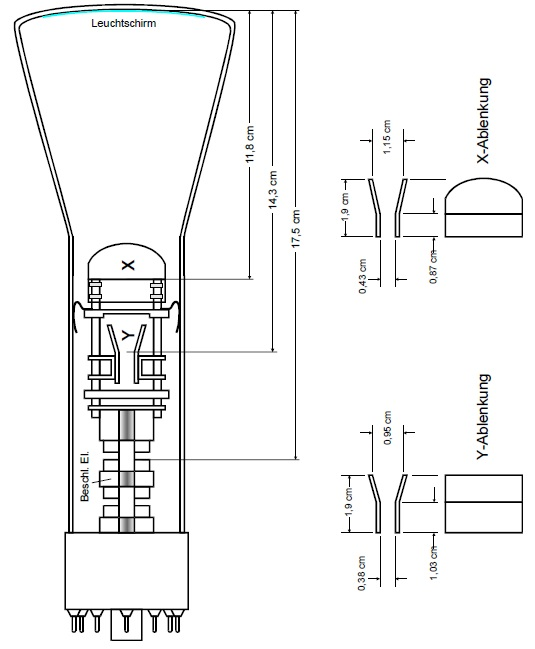
\includegraphics[width=0.7\textwidth, angle=270]{Grafiken/V501(2)_Abb3.jpg}
  \caption{Darstellung der Kathodenstrahlröhre }
\end{figure}

\subsubsection{Kathodenstrahl-Oszillograph}
Mit dem Kathodenstrahl-Oszillographen kann nun die Zeitabhängigkeit von Wechselspannungen dargestellt werden.  Es wird nun an das in X-Richtung ablenkende Plattenpar eine Sägezahnspannung angelegt und an die vertikal ablenkenden Platten (Y-Richtung) wird die zu untersuchende Spannung angelegt. Wenn die Sägezahn- und die Wechselspannung nun in einem geeigneten Verhältnis (\ref{eq:Theorie_freqVerhältnis})
 zueinander, zeichnet der Elekronenstrahl den zeitlichen Verlauf der Wechselspannung auf dem Leuchtschirm(kartesisches Koordinatensystem) ab.

\subsection{E-Feld}

Für ein festes $U_B$ werden die Ablenkspannungen gemessen, die die Verschiebung des Leuchtpunkts genau auf eine der Gitternetzlinien (Abstand $\frac{1}{4}$ inch.) auf dem Schirm bewirken. Dieser Vorgang wird für
fünf verschiedene Beschleunigungsspannungen wiederholt.
Danach werden zwei Funktionen durch einen Funktionengenerator erzeugt, diese auf die X- und Y-Eingänge gelegt und die Frequenzen gemessen, bei denen sich das Verhältnis 

\begin{equation}
\label{eq:Theorie_freqVerhältnis}
n \cdot \nu_\text{Sägezahn} = m \cdot \nu_\text{Sinus} \quad n, m\in\mathbb{N}
\end{equation}

einstellt.

\subsection{B-Feld}

Ein homogenes Magnetfeld wird mit Hilfe eines Helmholtzspulenpaares erzeugt. Zunächst muss
mit einem Inklinatorium die Richtung der Horizontalkomponente des Erdmagnetfelds bestimmt und die
Messapparatur in diese Richtung gedreht werden, damit das Erdmagnetfeld den Versuch nicht beeinflusst.
Danach wird mit konstanter Beschleunigungsspannung die Strahlverschiebung in Abhängigkeit vom Magnetfeld gemessen, das bei einem Helmholtz-Spulenpaar vom durchfließenden Strom abhängt.

\begin{equation}
\label{eq:Theorie_Magnetfeld}
B = \mu_0\frac{8 N I}{\sqrt{125}R}
\end{equation}

Dabei ist N die Windungszahl (hier: 20) und R den Spulenradius (hier: 0,282 m).
Des Weiteren wird die Stärke des Erdmagnetfelds durch Ausrichten des Leuchtpunkts auf die Mitte des Schirms und dann durch Drehen des Versuchsaufbaus um 90° bestimmt. Dabei verschiebt sich der Elektronenstrahl. Nun wird das von der Helmholtz-Spule erzeugte Magnetfeld
gerade so hoch geregelt, dass der Elektronenpunkt in der Mitte des Schirms ist. Aus diesem Wert des Magnetfeldes und dem Inklinationswinkel des Erdmagnetfelds, der ebenfalls mit dem Inklinatorium bestimmt wird, kann man die Stärke des Erdmagnetfelds errechnen.

Vor Beginn der Messung wird die Achse der Kathodenstrahlröhre nach
Norden ausgerichtet. Zum Auffinden dieser Richtung wird ein
Inklinatorium-Deklinatorium benutzt. Dann wird einmal bei
\SI{250}{\volt} Beschleunigungsspannung und einmal bei \SI{450}{\volt}
die Leuchtpunktverschiebung in Abhängigkeit des Spulenstroms gemessen.

\subsection{Bestimmung der Stärke des Erdmagnetfeldes}

Die Achse der Röhre wird wieder nach Norden ausgerichtet. Bei einer
Beschleunigungsspannung von \SI{200}{\volt} betrachtet man den
Leuchtschirm und merkt sich die Lage des Leuchtpunktes. Dann wird die
Anordnung um $\pi/2$ gedreht, so dass die Achse der Röhre in
Ost-West-Richtung zeigt. Nun muss mit dem Feld der
Helmholtz-Spulen der Leuchtpunkt so abgelenkt werden, dass er in
der vorherigen Lage erscheint. Jetzt gleicht das Feld der Spulen das
horizontale Magnetfeld der Erde genau aus.

Um die Größe der Erdmagnetfeldstärke zu bestimmen, muss nur noch der
Inclinationswinkel $\varphi$ (zwischen Tangentialebene und Richtung des
Erdmagnetfeldes) bekannt sein. Dieser kann wieder mit dem
Inklinatorium-Deklinatorium bestimmt werden. Zunächst wird die
Nord-Süd-Richtung mit dem Deklinatorium aufgefunden, dann der Teilkreis
um $\pi/2$ gedreht. Jetzt kann der Winkel abgelesen werden.
